%-----------------------------------------------------
% Chapter: Methodology
%-----------------------------------------------------
\chapter{Methodology}
This chapter details the methodology 
\label{chap:data_methodology}
\section{Collecting Data}
As previously mentioned, there exists no central repository from which song lyrics can be obtained. Though lyric hosting websites such as Genius\footnote{https://genius.com/} exist, selective collection of song lyrics is only achievable through the process of web scraping. Web scraping is the process of exhaustively downloading web pages, using a predefined list of URLs or through link extraction/following. Large scale web scraping is usually achieved through parallelised methods due to restrictions such as robots exclusion protocol (\textit{Robots.txt}) and download latency. Taking into account the project objectives and goals, web scraping was unfavourable and hence avoided.

\noindent
\newline
To overcome the issue of data availability, a public dataset containing over 250,000 lyrics was used(LINK TO DATASET). The dataset comprised of two .csv files: artists and lyrics. The artists .csv file mapped individual artists to their respective genres/sub genres, whilst the lyrics .csv file contained data on individual songs, mapping song lyrics to artists. 
\section{Data Analysis and Restructuring}
The CoVeR algorithm requires sub corpora to be labelled in order to jointly learn word embeddings and the relevant transformation matrices. With that in mind, a mapping between song lyrics and genre was required. To fulfil this requirement Pandas, a Python data analysis library, was used to perform a SQL like join on the artist column contained in both files.

\noindent
\newline
A trivial approach to split the lyric corpora on genre would involve an equal split for equal representation, however, this method uses the assumption that for each genre, song lyrics contain equivalent amounts of words. Examining the dataset however, proved this not to be the case.

\begin{figure}[h]
	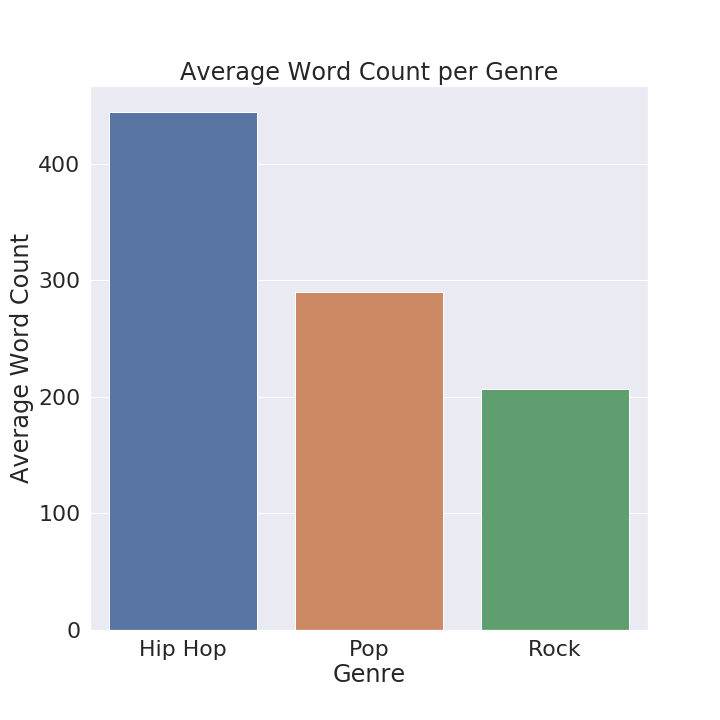
\includegraphics[width=8cm, height=8cm]{./figures/fig6}
	\centering
	\caption{Average word count per lyric per genre in the dataset}
	\label{fig:fig6}
\end{figure}

\noindent
\newline
Analysing the dataset, the mean number of words contained in a Hip-Hop song was 444; being more than double the mean number of words found in Rock songs which was 207. Regarding Pop songs, the mean word count was 289. To reflect these statistics and also due to constraints in the distribution of data by genre, 100,000 song lyrics were randomly selected to create the dataset to be used to train CoVeR. Moreover a data split of 48:30:22 for Rock, Pop and Hip-Hop, was to maintain an even distribution of words by song genre within the dataset.
\section{Data Pre-processing}
Essential to any machine learning task is the pre-processing of input data in such a way that important features are accessible during training. In natural language processing, this can include techniques such as tokenisation, string cleaning, stemming and lemmatisation. 

\noindent
\newline
Following data reconstruction, each song lyric in the corpora was cleansed and tokenised. The following string cleaning techniques were applied to each lyric in the dataset.

\begin{enumerate}
	\item All letters were lowercased.
	\item All characters, except for letters, were substituted with a space " ".
	\item All text between brackets were removed. (This was to ensure text like \textbf{[Verse 1]} was not included during training).
	\item All trailing white space was removed.
\end{enumerate}

\noindent
\newline
Tokenisation is the process of separating textual inputs into meaningful chunks called \textit{tokens}. Naturally to create word embeddings, text is tokenised at the word level and each token assigned a unique integer key, representing that token numerically. For training, only tokens which appeared at least 30 times were kept. Moreover for only the top 15,000 words were considered.
 
\noindent
\newline
Typically found within text corpora are high frequency stop words such as which provide less information than rarely occurring words (\cite{Mikolov2013a}). For example... This concept can also be applied to word embeddings; where the word embeddings of frequent words does not change significantly after training on several examples. Taking inspiration from word2vec, subsampling was used at the covariate level using the following adapted formula from the original word2vec implementation.

\begin{equation}
P(w_{ik}) = \sqrt{\dfrac{z(w_{ik})}{t}} + 1 \cdot \dfrac{t}{z(w_{ik})}
\end{equation}

\noindent
\newline
where \(z(w_{ik})\) is the percentage of word \(w_{ik}\) in covariate \(k\) and \(t\) is a chosen threshold.

\section{Hyper-parameters}
Hyper-parameters within machine learning models are parameters that govern a given model. The selection of these parameters directly impacts the performance of a given training algorithm and as such, optimal hyper-parameter choice is important for producing optimal performance for a given model. Both CoVeR and LSTM networks have important hyper-parameters which are reviewed in the following section.
\subsection{CoVeR Hyperparamters}
\subsubsection{Context Windows}
Like GloVe, CoVeR also uses weighted context windows during the process of calculating co-occurrence statistics. The CoVeR paper uses a context window size of 8, however the paper does not specify whether they used symmetric or asymmetric windows during their experiments. As such, both are experimented with whilst performing hyperparameter tuning.  
\subsubsection{Embedding Size}
\subsubsection{Optimiser}
\subsubsection{Hyperparameter Tuning}
\subsection{LSTM Hyperparameters}
\subsubsection{Dropout}
Dropout is a regularization technique proposed by \cite{Srivastava2014}, which involves the random dropping of nodes and their connections within a network. Selected nodes are picked at random using a probability known as the dropout rate. Dropout helps to decrease over-fitting as 
\subsubsection{Embedding Layer}
\subsubsection{Optimiser}

